\chapter{Digital-Analog Wandler / Analog-Digital Wandler}
\textbf{Beispiel Musikspeicherung} \\
Schwallwellen $\rightarrow$ Mikrophon (Spannung - analoges Signal) $\rightarrow$ MP3-Datei (Bit 0/1 - digitales Signal) $\rightarrow$ DA-Wandler $\rightarrow$ Lautsprecher (analoges Signal)

\begin{figure}[H]
	\centering
	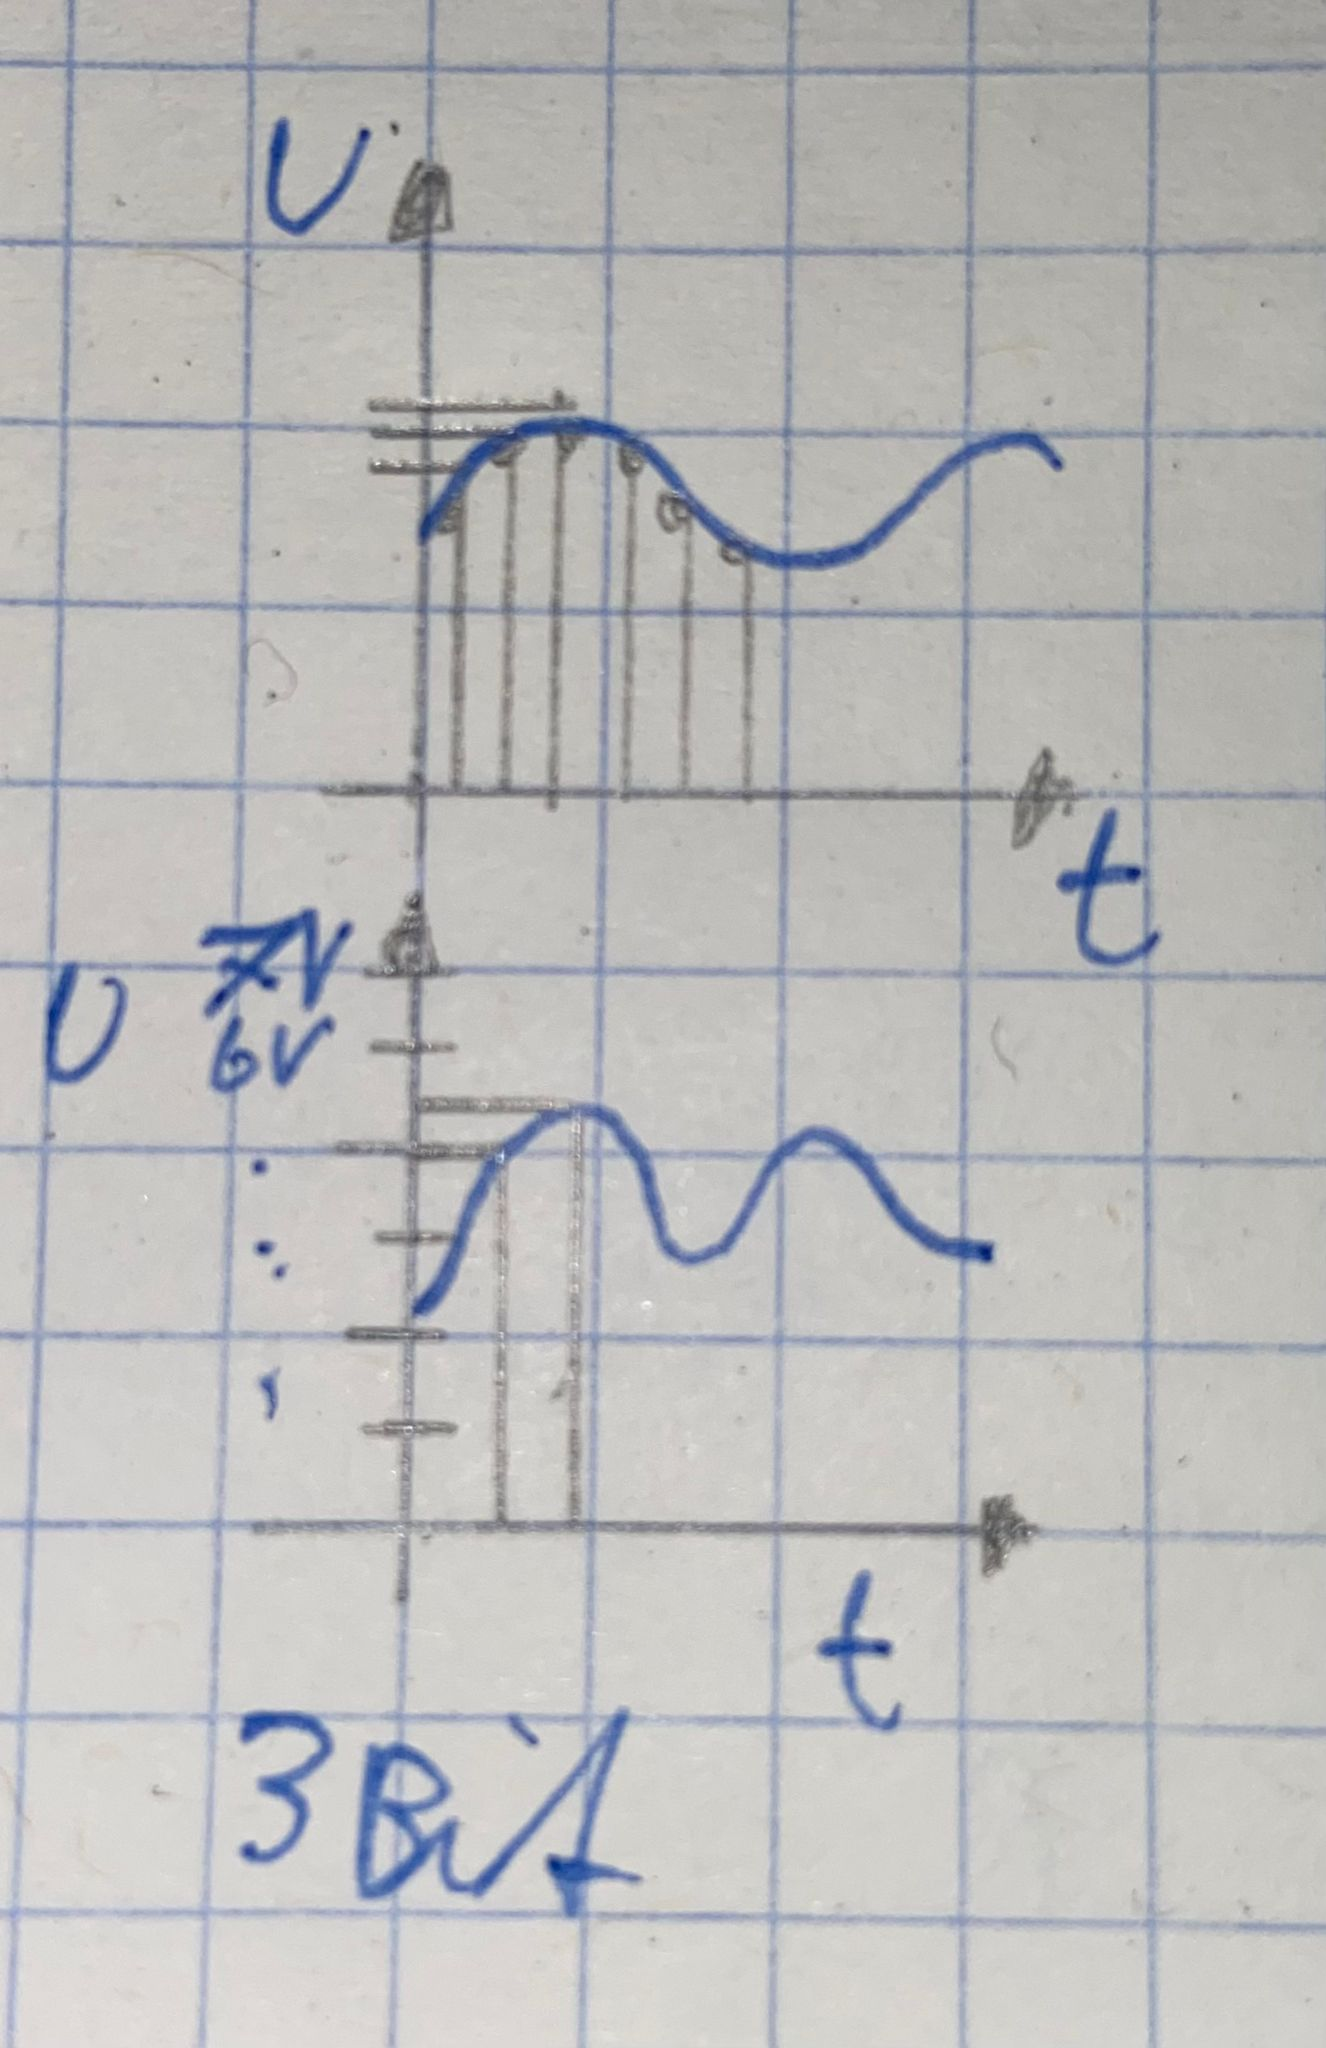
\includegraphics[width=0.2\linewidth]{figures/daad1.jpeg}
	\caption{DA/AD-Wandler}
\end{figure}

\begin{itemize}
	\item Pegel messen
	\item Binärzahl speichern
	\item je höher die Abtastrate (Samplerate) desto besser
	\item je mehr Bits zum Speichern verwendet werden, desto genauer
\end{itemize}
Typische Abtastrate: ca. 44 kHz

\textbf{Digital-Analog Wandler} \\
Aufgabe: muss aus einer Binärzahl eine Spannung erzeugen









